\documentclass[tikz,border=12pt]{standalone}
\usepackage[T1]{fontenc}
\usepackage{tgheros}
\usepackage{sfmath}
\usepackage{amsmath}
\usepackage{tikz}
\usetikzlibrary{arrows.meta,positioning,shapes.geometric,fit,backgrounds,calc}
\usepackage{xcolor}

\renewcommand{\familydefault}{\sfdefault}

% Academic Semantic Palette
\definecolor{harvardcrimson}{HTML}{A51C30}
\definecolor{ethdarkblue}{HTML}{1F407A}
\definecolor{ethblue}{HTML}{215CAF}
\definecolor{ethpetrol}{HTML}{007A87}
\definecolor{ethbronze}{HTML}{B87333}
\definecolor{ethpurple}{HTML}{5B4B8A}
\definecolor{ethslate}{HTML}{475569}
\definecolor{cardbg}{HTML}{F8FAFC}
\definecolor{cardborder}{HTML}{CBD5E1}
\definecolor{safeTeal}{HTML}{10B981}
\definecolor{amberProp}{HTML}{C98218}
\definecolor{amberBg}{HTML}{FFF3DC}
\definecolor{coralVeto}{HTML}{BD4F2F}
\definecolor{coralBg}{HTML}{FAE9E2}
\definecolor{navyBg}{HTML}{E8EDF6}
\definecolor{tealBg}{HTML}{E4F6F3}

\begin{document}
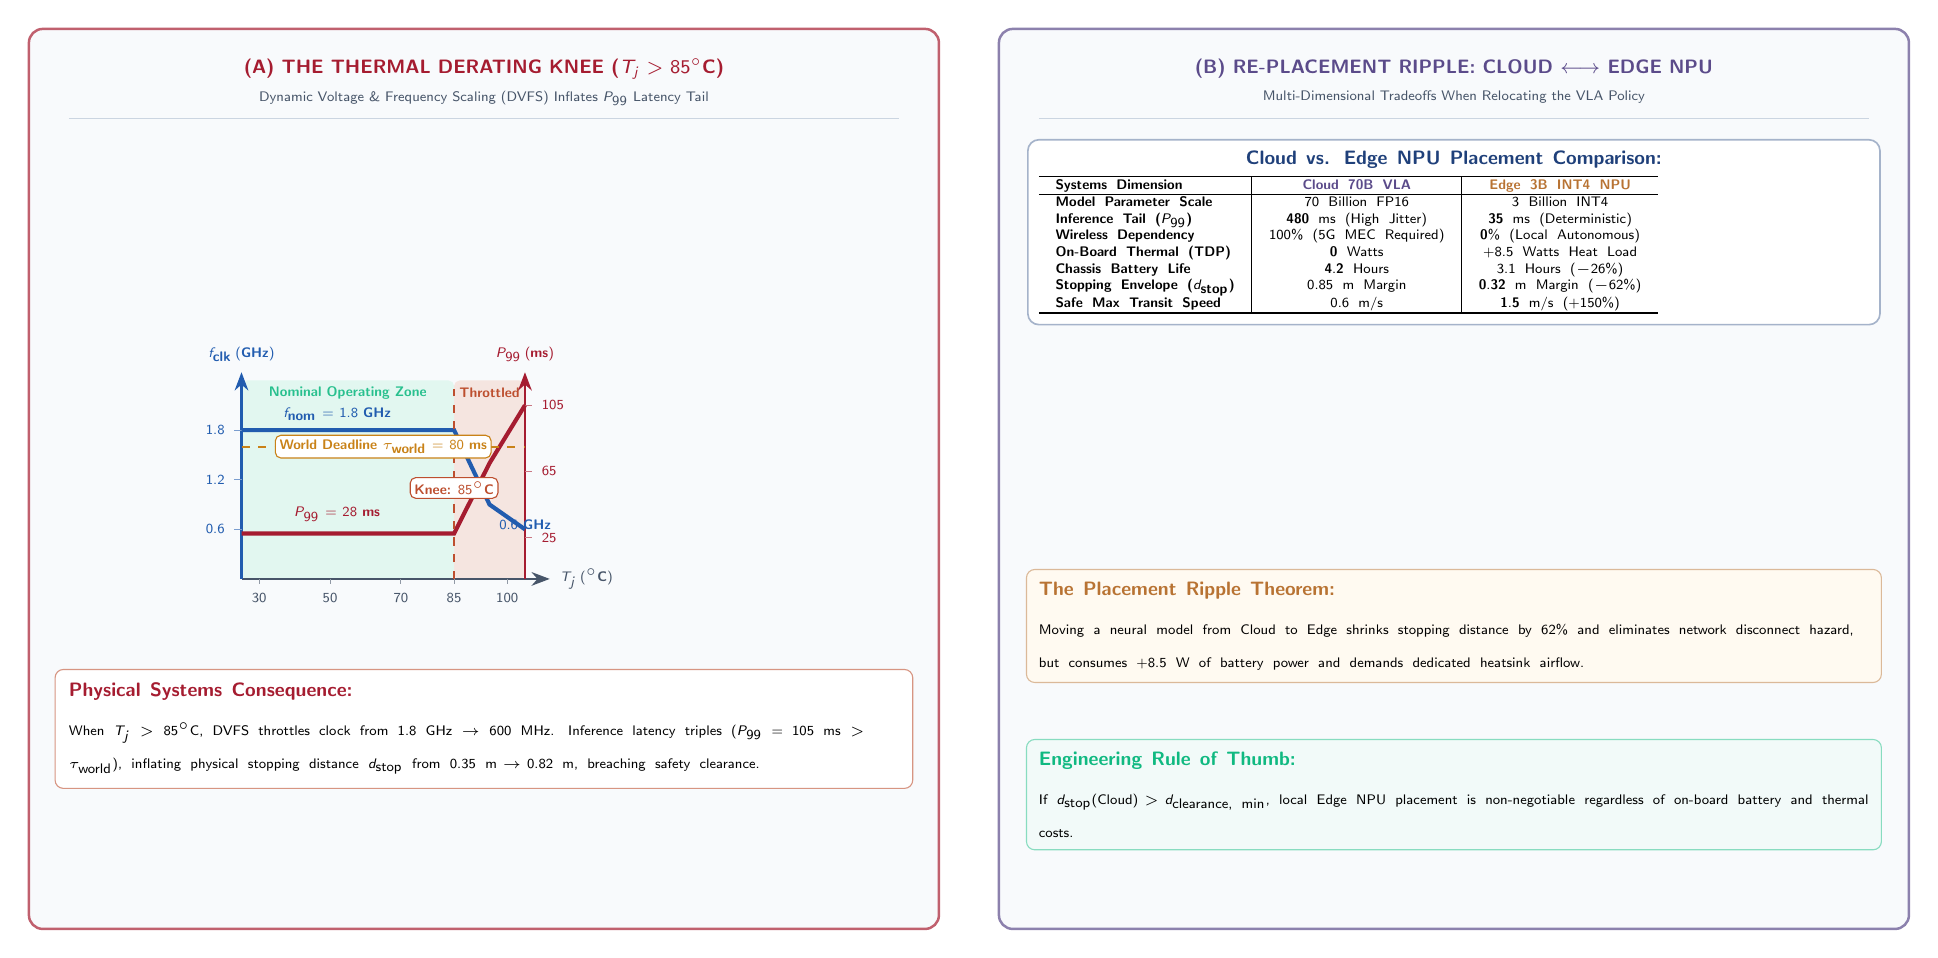
\begin{tikzpicture}[
  font=\sffamily,
  >=Stealth
]

  % ====================================================
  % PANEL A: THE THERMAL DERATING KNEE (Left)
  % ====================================================
  \draw[draw=harvardcrimson!70, fill=cardbg, rounded corners=5pt, line width=0.9pt]
    (0, 0) rectangle ++(4.55in, -4.50in);

  \node[anchor=north, font=\scriptsize\bfseries, color=harvardcrimson] at (2.275in, -0.10in) {
    (A) THE THERMAL DERATING KNEE ($T_j > 85^\circ\text{C}$)
  };
  \node[anchor=north, font=\tiny, color=ethslate] at (2.275in, -0.26in) {
    Dynamic Voltage \& Frequency Scaling (DVFS) Inflates $P_{99}$ Latency Tail
  };
  \draw[draw=cardborder, line width=0.4pt] (0.20in, -0.45in) -- (4.35in, -0.45in);

  % Graph inside Panel A
  \begin{scope}[shift={(0.62in, -2.75in)}, xscale=0.045, yscale=1.05]
    % Background zones
    \draw[fill=safeTeal!12, draw=none, rounded corners=2pt] (25, 0) rectangle (85, 2.4);
    \draw[fill=coralVeto!15, draw=none, rounded corners=2pt] (85, 0) rectangle (105, 2.4);
    
    \node[font=\tiny\bfseries, text=safeTeal!90] at (55, 2.25) {Nominal Operating Zone};
    \node[font=\tiny\bfseries, text=coralVeto] at (95, 2.25) {Throttled};

    % Axes
    \draw[->, line width=0.8pt, draw=ethslate] (25, 0) -- (112, 0) node[right, font=\tiny\bfseries, text=ethslate] {$T_j\,(^\circ\text{C})$};
    \draw[->, line width=0.8pt, draw=ethblue] (25, 0) -- (25, 2.5) node[above, font=\tiny\bfseries, text=ethblue] {$f_{\text{clk}}\,(\text{GHz})$};
    \draw[->, line width=0.8pt, draw=harvardcrimson] (105, 0) -- (105, 2.5) node[above, font=\tiny\bfseries, text=harvardcrimson] {$P_{99}\,(\text{ms})$};

    % Ticks X
    \foreach \t in {30, 50, 70, 85, 100} {
      \draw[draw=ethslate!60] (\t, 0) -- (\t, -0.06);
      \node[below, font=\tiny, text=ethslate] at (\t, -0.06) {\t};
    }

    % Ticks Left Y (f_clk)
    \draw[draw=ethblue!60] (25, 0.6) -- (23, 0.6);
    \node[left, font=\tiny, text=ethblue] at (23, 0.6) {0.6};
    \draw[draw=ethblue!60] (25, 1.2) -- (23, 1.2);
    \node[left, font=\tiny, text=ethblue] at (23, 1.2) {1.2};
    \draw[draw=ethblue!60] (25, 1.8) -- (23, 1.8);
    \node[left, font=\tiny, text=ethblue] at (23, 1.8) {1.8};

    % Ticks Right Y (P99 Latency)
    \draw[draw=harvardcrimson!60] (105, 0.5) -- (107, 0.5);
    \node[right, font=\tiny, text=harvardcrimson] at (107, 0.5) {25};
    \draw[draw=harvardcrimson!60] (105, 1.3) -- (107, 1.3);
    \node[right, font=\tiny, text=harvardcrimson] at (107, 1.3) {65};
    \draw[draw=harvardcrimson!60] (105, 2.1) -- (107, 2.1);
    \node[right, font=\tiny, text=harvardcrimson] at (107, 2.1) {105};

    % Curves
    % Clock (blue)
    \draw[line width=1.5pt, draw=ethblue] (25, 1.8) -- (85, 1.8) -- (95, 0.9) -- (105, 0.6);
    \node[font=\tiny\bfseries, text=ethblue, above] at (52, 1.8) {$f_{\text{nom}} = 1.8\text{ GHz}$};
    \node[font=\tiny\bfseries, text=ethblue, right] at (95, 0.65) {$0.6\text{ GHz}$};

    % Latency (red)
    \draw[line width=1.5pt, draw=harvardcrimson] (25, 0.55) -- (85, 0.55) -- (95, 1.4) -- (105, 2.1);
    \node[font=\tiny\bfseries, text=harvardcrimson, above] at (52, 0.58) {$P_{99} = 28\text{ ms}$};

    % Knee Marker
    \draw[dashed, line width=1.0pt, draw=coralVeto] (85, 0) -- (85, 2.3);
    \node[font=\tiny\bfseries, fill=white, draw=coralVeto, rounded corners=2pt, inner sep=1.5pt, text=coralVeto] at (85, 1.1) {Knee: $85^\circ\text{C}$};

    % World Deadline Threshold
    \draw[dashed, line width=0.8pt, draw=amberProp] (25, 1.6) -- (105, 1.6);
    \node[font=\tiny\bfseries, fill=white, draw=amberProp, rounded corners=2pt, inner sep=1.5pt, text=amberProp] at (65, 1.6) {World Deadline $\tau_{\text{world}} = 80\text{ ms}$};
  \end{scope}

  % Systems Consequence Box inside Panel A
  \node[draw=coralVeto!60, fill=white, rounded corners=3pt, text width=4.15in, inner sep=5pt, align=left, anchor=north] at (2.275in, -3.20in) {
    {\scriptsize\bfseries\color{harvardcrimson} Physical Systems Consequence:}\\[2pt]
    {\tiny
    When $T_j > 85^\circ\text{C}$, DVFS throttles clock from $1.8\text{ GHz} \to 600\text{ MHz}$. Inference latency triples ($P_{99} = 105\text{ ms} > \tau_{\text{world}}$), inflating physical stopping distance $d_{\text{stop}}$ from $0.35\text{ m} \to 0.82\text{ m}$, breaching safety clearance.
    }
  };

  % ====================================================
  % PANEL B: RE-PLACEMENT RIPPLE (Right)
  % ====================================================
  \draw[draw=ethpurple!70, fill=cardbg, rounded corners=5pt, line width=0.9pt]
    (4.85in, 0) rectangle ++(4.55in, -4.50in);

  \node[anchor=north, font=\scriptsize\bfseries, color=ethpurple] at (7.125in, -0.10in) {
    (B) RE-PLACEMENT RIPPLE: CLOUD $\longleftrightarrow$ EDGE NPU
  };
  \node[anchor=north, font=\tiny, color=ethslate] at (7.125in, -0.26in) {
    Multi-Dimensional Tradeoffs When Relocating the VLA Policy
  };
  \draw[draw=cardborder, line width=0.4pt] (5.05in, -0.45in) -- (9.20in, -0.45in);

  % Comparison Table inside Panel B
  \node[draw=ethdarkblue!40, fill=white, rounded corners=4pt, line width=0.6pt, text width=4.15in, inner sep=4pt, anchor=north] (b_tab) at (7.125in, -0.55in) {
    \centering
    {\scriptsize\bfseries\color{ethdarkblue}Cloud vs. Edge NPU Placement Comparison:}\\[2pt]
    \tiny
    \begin{tabular}{l|c|c}
      \hline
      \textbf{Systems Dimension} & \textbf{\color{ethpurple}Cloud 70B VLA} & \textbf{\color{ethbronze}Edge 3B INT4 NPU} \\
      \hline
      \textbf{Model Parameter Scale} & $70\text{ Billion FP16}$ & $3\text{ Billion INT4}$ \\
      \textbf{Inference Tail ($P_{99}$)} & $\mathbf{480\text{ ms}}$ (High Jitter) & $\mathbf{35\text{ ms}}$ (Deterministic) \\
      \textbf{Wireless Dependency} & $100\%$ (5G MEC Required) & $\mathbf{0\%}$ (Local Autonomous) \\
      \textbf{On-Board Thermal (TDP)} & $\mathbf{0\text{ Watts}}$ & $+8.5\text{ Watts}$ Heat Load \\
      \textbf{Chassis Battery Life} & $\mathbf{4.2\text{ Hours}}$ & $3.1\text{ Hours}$ ($-26\%$) \\
      \textbf{Stopping Envelope ($d_{\text{stop}}$)} & $0.85\text{ m}$ Margin & $\mathbf{0.32\text{ m}}$ Margin ($-62\%$) \\
      \textbf{Safe Max Transit Speed} & $0.6\text{ m/s}$ & $\mathbf{1.5\text{ m/s}}$ ($+150\%$) \\
      \hline
    \end{tabular}
  };

  % Summary Callout 1 in Panel B
  \node[draw=ethbronze!50, fill=amberBg!40, rounded corners=3pt, text width=4.15in, inner sep=4.5pt, align=left, anchor=north] at (7.125in, -2.70in) {
    {\scriptsize\textbf{\color{ethbronze} The Placement Ripple Theorem:}}\\[2pt]
    {\tiny Moving a neural model from Cloud to Edge shrinks stopping distance by $62\%$ and eliminates network disconnect hazard, but consumes $+8.5\text{ W}$ of battery power and demands dedicated heatsink airflow.}
  };

  % Summary Callout 2 in Panel B
  \node[draw=safeTeal!50, fill=tealBg!50, rounded corners=3pt, text width=4.15in, inner sep=4.5pt, align=left, anchor=north] at (7.125in, -3.55in) {
    {\scriptsize\textbf{\color{safeTeal} Engineering Rule of Thumb:}}\\[2pt]
    {\tiny If $d_{\text{stop}}(\text{Cloud}) > d_{\text{clearance, min}}$, local Edge NPU placement is non-negotiable regardless of on-board battery and thermal costs.}
  };

\end{tikzpicture}
\end{document}
